%----------------------------------------------------------------
%
%  File    :  thesis-struc.tex
%
%  Author  :  Keith Andrews, IICM, TU Graz, Austria
% 
%  Created :  27 May 93
% 
%  Changed :  19 Feb 2004
% 
%----------------------------------------------------------------


\chapter{Structuring a Thesis}

\label{chap:Struc}

\chapquote{
Tell them what you are going to tell them. \\
Tell them. \\
Tell them what you told them.
}
{
Age-old adage for successful presentation.
}




Every chapter and every section should have some introductory text at
the beginning, like this text. Never jump straight in to the first
secion or subsection without one or more paragraphs of introductory
text.




\section{Pyramid Writing Structure}

Bear in mind that most of the readers of a thesis will have very
limited time. Most will only read the title and abstract. Some may
read the Introduction and Concluding Remarks. A few will read one or
two particular chapters. Only a very select few will actually read the
whole thesis from start to finish.


\begin{figure}[tp]
\centering
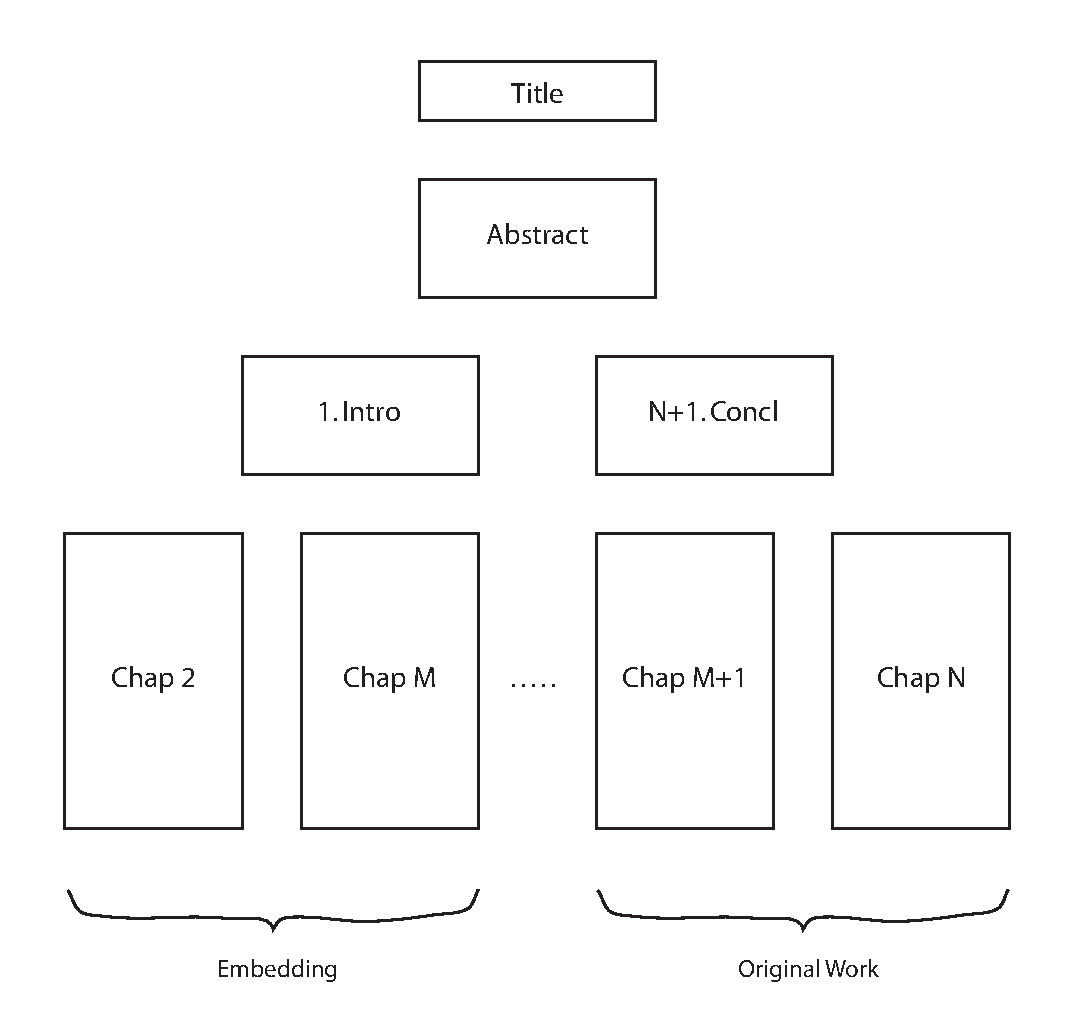
\includegraphics[keepaspectratio,width=\linewidth,height=\halfh]
{diagrams/pyramid.pdf}

\caption[Pyramid Writing Structure]{
Using a pyramid to structure a thesis into self-contained chunks
of increasing detail.
\imgcredit{Image drawn by the author of this thesis.}
}
\label{fig:Pyramid}
\end{figure}


The lesson from this is to structure your thesis as a pyramid in
self-contained units of increasing detail, as illustrated in
Figure~\ref{fig:Pyramid}. The main structural units are:
\begin{itemize}
\item \textbf{Title} \\
The title should be self-contained and comprise a good set of
representative keywords. Representative keywords in the title help
your work be found by an electronic search.

\item \textbf{Abstract} \\
The abstract should compactly, in two or three paragraphs, describe
the motivation for the work (embedding and context), what was done, and
the results and contributions (what is really new). As a rule of
thumb: the abstract summarises the thesis with about one sentence
corresponding to each chapter of the thesis.


\item \textbf{1. Introduction} \\
``Tell them what you are going to tell them''. As a rule of thumb: the
introduction contains one paragraph of text for each chapter in the
body of the thesis. Emphasise any original work and contributions.

\item \textbf{2. Embedding} \\
Two or three chapters embedding the thesis in the context of related
work, including an extensive literature survey.

\item \textbf{Chapter M}

\item \textbf{Chapter M+1} \\
Chapters containing the original work of the author.

\item \textbf{Chapter N}

\item \textbf{Concluding Remarks} \\
``Tell them what you told them''. One paragraph of text summarising
what was presented in each chapter of the body of the thesis.
Emphasise your own original work and achievements.

\item \textbf{Appendices} \\
Optional appendices might include a User Guide and a Developer
Guide, when software has been written as part of the thesis project.

\item \textbf{Bibliography} \\
There is some debate as to whether the bibliography should
be placed before or after any appendices. Many prefer after,
so that references can be looked up more easily. Others
prefer before, especially if there are extensive appendices.
If in doubt, ask your supervisor.

\end{itemize}




\section{Composing a Title and Abstract}

One useful strategy for composing a good title and abstract involves
brainstorming for a list of keywords. Start by writing down a list of
all the words and phrases describing important topics covered in the
thesis and which potential interested readers might use as search
terms to find the thesis. Then construct a title containing the most
important of these keywords. Finally, compose the abstract and make
sure most of the rest of the keywords are contained somewhere in the
abstract. Search engines and library systems will usually index the
title and the abstract, so anyone searching for any of the keywords
should now be able to find the thesis. When the thesis is approaching
completion, revisit the title and abstract, an extra extra keywords
and make any necessary adaptations.




\section{Double-Sided Printing}

Create and print your thesis in colour and for two-sided (duplex)
printing. Modern laser printers can easily handle printing out in
colour and double-sided. A thesis printed one-sided will be
(unnecessarily) twice as thick and twice as heavy.

Chapters, including the bibliography and any appendices, must
\emph{always} start on a new right-hand (odd-numbered) page.  This is
what the \lstinline!\cleardoublepage! command does.






\section{Single Children}

As in real life, a single child is not a good idea. A chapter with
only one section makes no sense. A section with only one subsection
makes no sense. A subsection with only one subsubsection makes no
sense either. If a structural unit has subunits, then there should
always be at least two subunits.







\section{Make Captions Carry the Story Too}

Some readers like to scan through your work from figure to figure,
gaining an impression of what it is about by reading the captions.
Support these readers by:
\begin{itemize}
\item \emph{Writing self-contained captions}: the caption
should describe the figure or table as completely as possible, without
assuming knowledge of material in the running text.

\item \emph{Writing longish captions}: it is fine for
captions to contain two or three sentences.

\item \emph{Stringing captions together}: Reading successive captions
should also tell an abridged version of the entire story.
\end{itemize}




\section{Avoid Orphan Floats}

Every floating element (figure, table, or listing) which appears in
the thesis and is given its own number such as Figure~3.1, Table~4.1,
or Listing~5.1 \emph{must} be discussed and referenced somewhere in
the running text. An orphan float is a float which appears and has a
number, but is never referenced in the flowing text.


